\chapter{Soluții similare}
\section{Prezentare generală a formatului PDF}

Portable Document Format (PDF) este un tip de fișier dezvoltat de Adobe în anul 1992. La baza acestui fișier stă PostScript, un limbaj de descriere a paginilor. Fiecare document PDF conține o descriere completă a structurii, a textului, a imaginilor și alte informații.

Formatul PDF oferă multe detalii despre fișier, ceea ce permite cu ușurință creearea de aplicații de convertire a documentelor în format HTML. Acestea există de mai bine de 26 ani \cite{kieninger1998paper} și folosesc diferite metode pentru a realiza transformarea. În capitolele următoare sunt analizate câteva dintre soluțiile de convertire existente, dar și motivele pentru care nu sunt adecvate în raport cu cerințele date de Minister.

Criteriile principale căutate sunt: posibilitatea de a selecta textul din fișierul HTML la afișare, paginile să fie responsive, codul să fie scris într-un mod ușor de editat.


\section{Conversia în imagini}

Metoda de conversie în imagini constă în transformarea paginilor din manuale PDF în imagini, urmată de inserarea acestora în fișiere HTML. Această metodă este simplă și rapidă din punct de vedere al implementării, dar nu îndeplinește cerințele cerute, deoarece textul nu poate fi selectat.

Pe lângă acest dezavantaj, mai apare și problema dimensiunii imaginilor. Transformarea paginilor în imagini are ca rezultat un folder director de dimensiuni mari care ar putea să depășească limita maximă admisă din caietul de sarcini.
\begin{figure}[H]
	\centering
	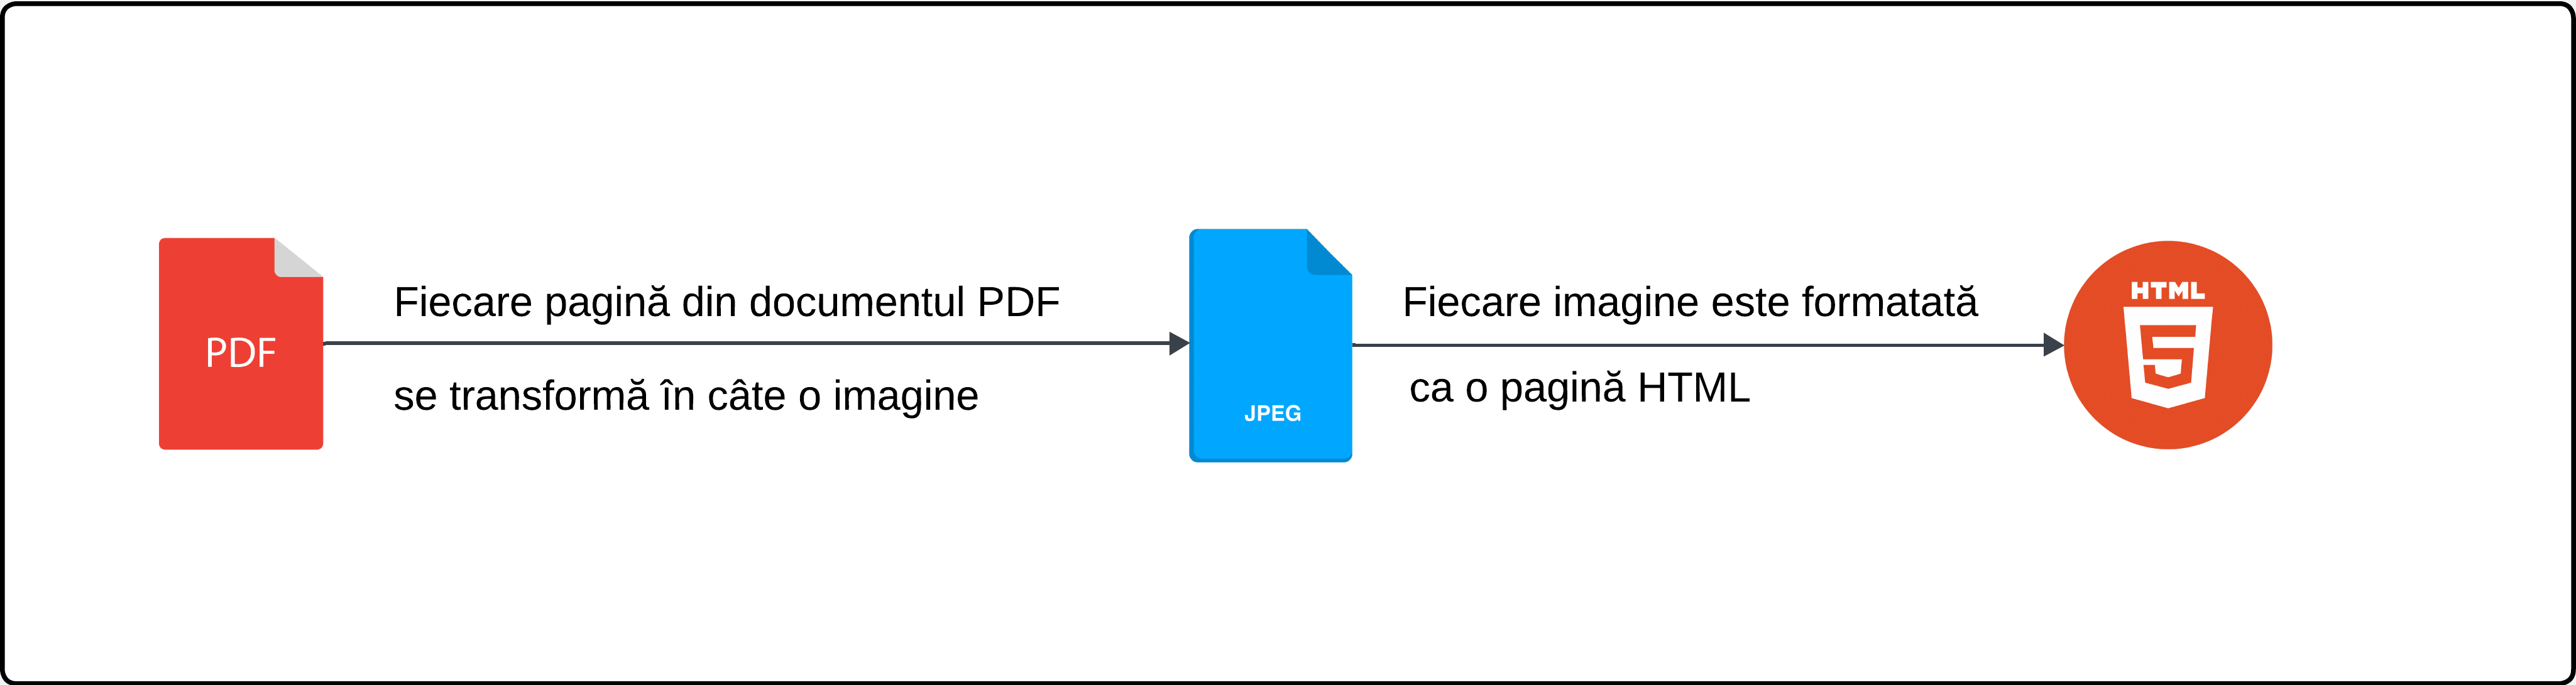
\includegraphics[scale=.4]{Figura2_1}
	\caption{Procesul de transformare a documentului PDF prin convertirea în imagini}
	\label{fig:Figura2_1}
\end{figure}


\section{Soluția de conversie de la Adobe Acrobat Pro}

Adobe Acrobat \cite{padova2008adobe} este o aplicație dezvoltată de Adobe, utilizată în toată lumea pentru crearea, manipularea, afișarea și gestionarea documentelor PDF.

Una dintre funcționalitățile sale este conversia documentelor PDF în format HTML, disponibilă numai în varianta cu plată a software-ului (Adobe Acrobat Pro). Acest lucru reprezintă un inconvenient pentru cazul de față.
\vspace{1em}

\noindent
Dezavantaje:
\begin{itemize}
	\item formatare greșită a textului;
	\item accesibil doar pentru varianta plătită.
\end{itemize}



\section{XHTML 1.0 Transitional}
\subsection{Soluția Xodo}

Extensible HyperText Markup Language (XHTML) \cite{musciano2006html} este un limbaj folosit pentru crearea și afișarea paginilor web. Acesta este foarte similar cu HTML (HyperText Markup Language), dar include câteva restricții suplimentare. XHTML este o versiune de HTML bazată pe formatul XML, care nu permite, de exemplu, lăsarea tagurilor deschise.

Xodo este un instrument care transformă documente PDF în format XHTML. Acesta permite o singură conversie gratuită pe zi și nu oferă rezultate bune. Structura documentului se desparte greșit și nu respectă culoarea de fundal.
\begin{figure}[H]
	\centering
	\begin{subfigure}{.5\textwidth}
		\centering
		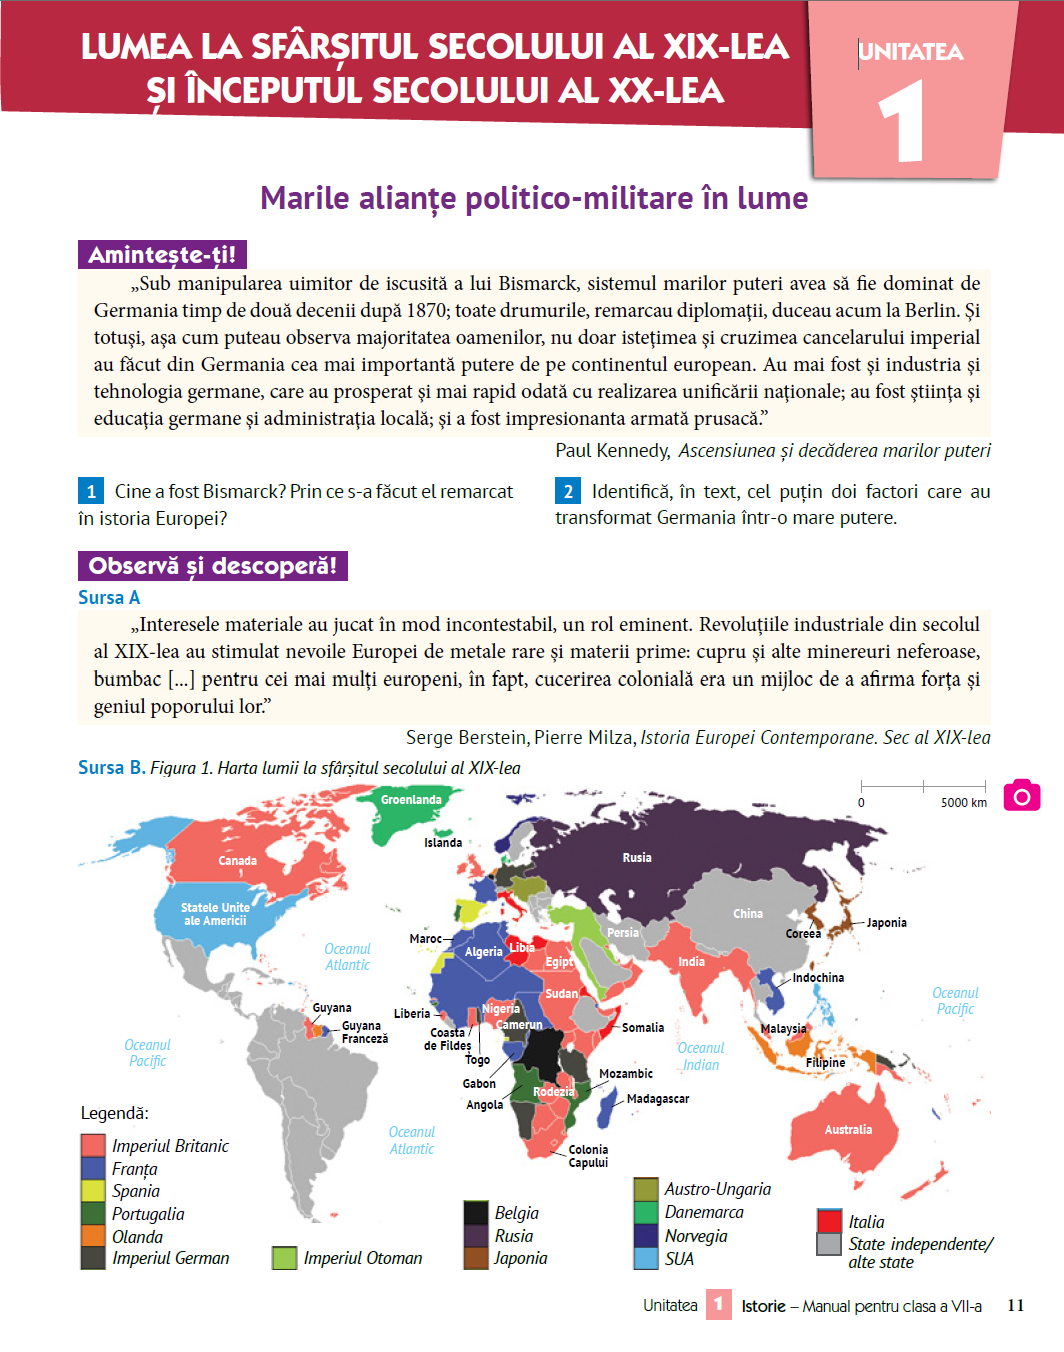
\includegraphics[width=.8\linewidth, height=.30\textheight]{Figura2_2a}
		\caption{pagină din manualul tipărit}
		\label{fig:Figura2_2a}
	\end{subfigure}%
	\begin{subfigure}{.5\textwidth}
		\centering
		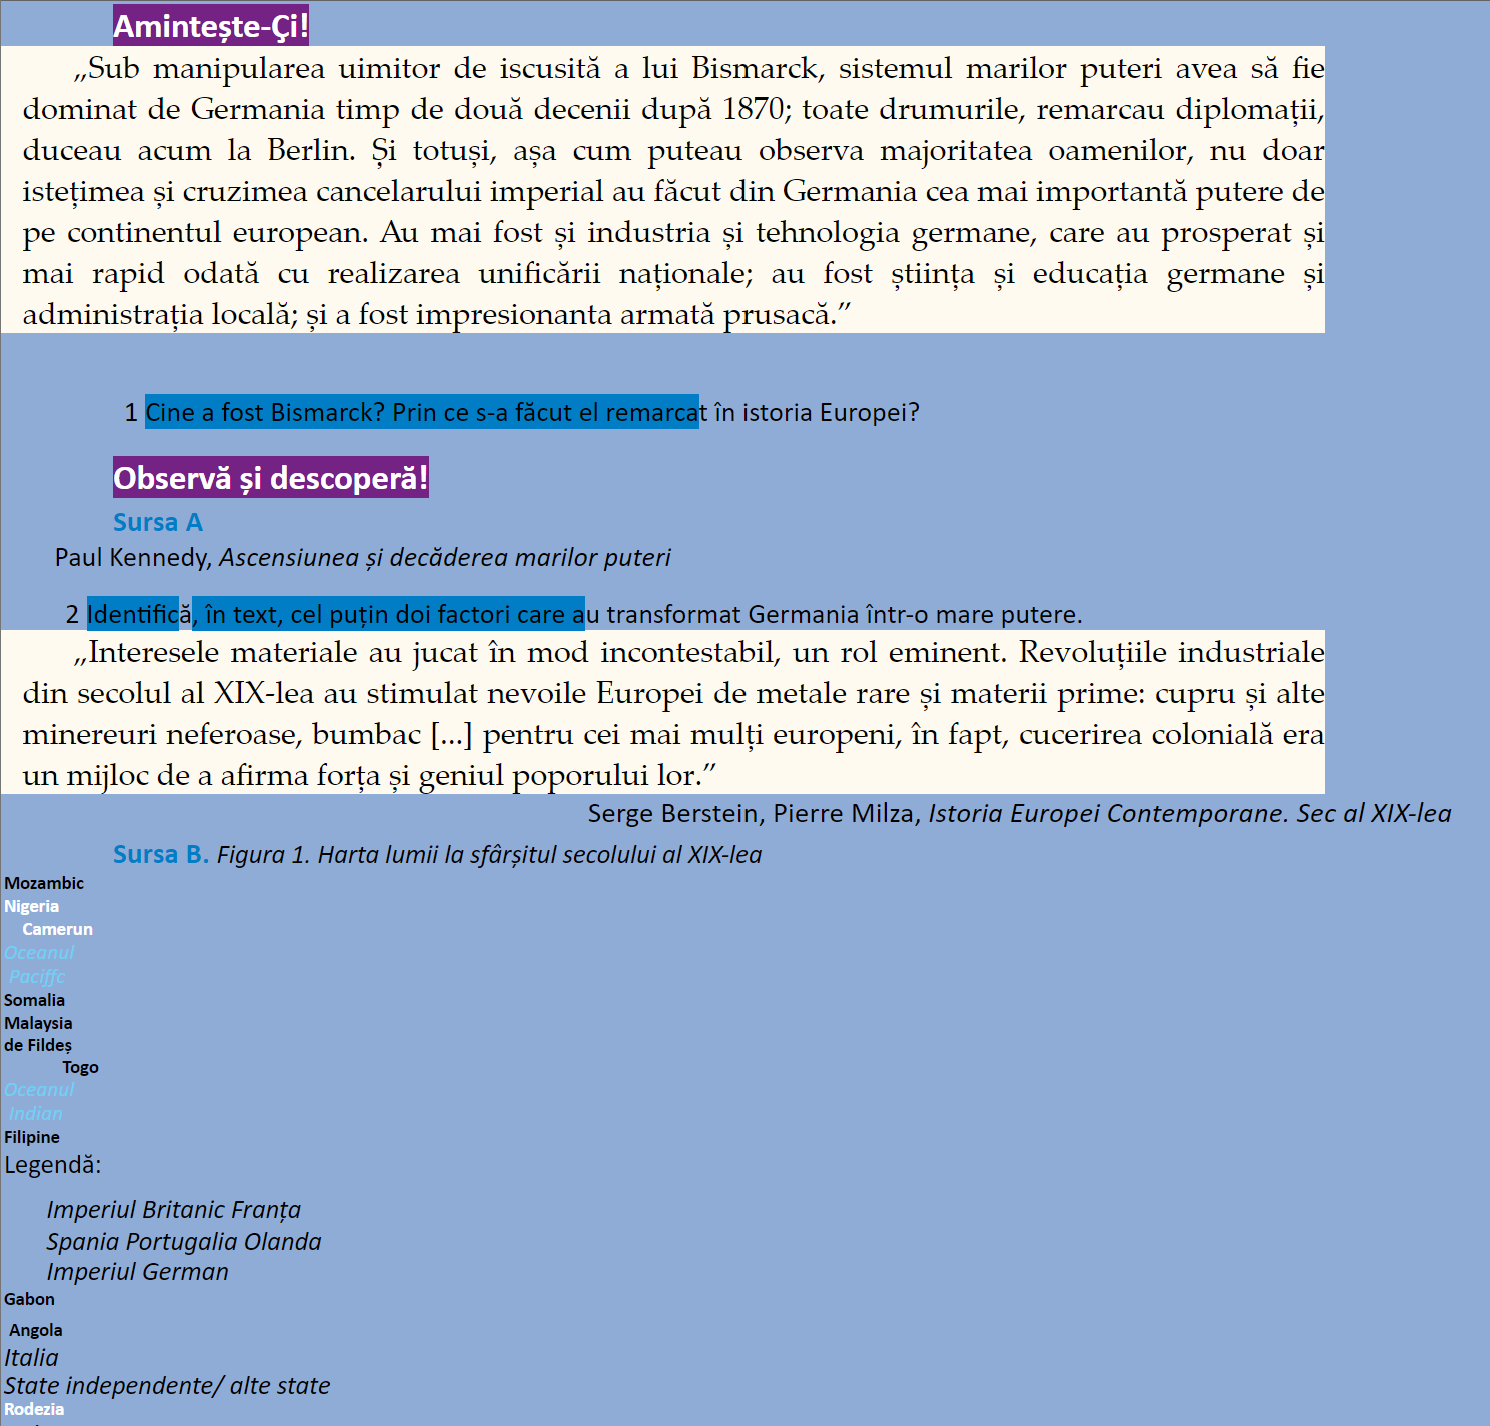
\includegraphics[width=.8\linewidth, height=.30\textheight]{Figura2_2b}
		\caption{pagină HTML generată de Xodo}
		\label{fig:Figura2_2b}
	\end{subfigure}
	\caption{Comparație de pagini dintre varianta tipărită și cea de la Xodo}
	\label{fig:Figura2_2}
\end{figure}

\noindent
Avantaje:
\begin{itemize}
	\item generează rapid pagini HTML;
	\item paginile sunt responsive;
	\item textul este selectabil.
\end{itemize}

\noindent
Dezavantaje:
\begin{itemize}
	\item limitat la o singură utilizare gratis pe zi;
	\item codul HTML este greu de editat;
	\item formatare greșită a textului.
\end{itemize}

\subsection{Soluția pdf2htmlEX}

O soluție care oferă o formatare ideală este obținută folosind pdf2htmlEX \cite{wang2013online}. Acest instrument păstrează tot textul și formatarea din PDF, dar are două dezavantaje. În primul rând, paginile rezultate nu sunt responsive, ceeea ce este o condiție obligatorie. O pagină responsive își păstrează structura atunci când este redimensionată. De exemplu, pagina HTML redimensionată pentru un ecran de telefon ar trebui să-și păstreze structura, ceea ce nu se întâmplă în cazul de față. Pe lângă acest lucru, codul HTML este greu de citit și de editat. O linie de cod poate să ajungă până la 60.000 de caractere. În cazul în care apar modificări în manual, acestea vor fi greu de editat.

Două dintre site-urile care folosesc acest instrument sunt CloudConvert și Convertio. Acestea dau rezultate asemănătoare, dar au amândouă aceleași probleme.
\begin{figure}[H]
	\centering
	\begin{subfigure}{.5\textwidth}
		\centering
		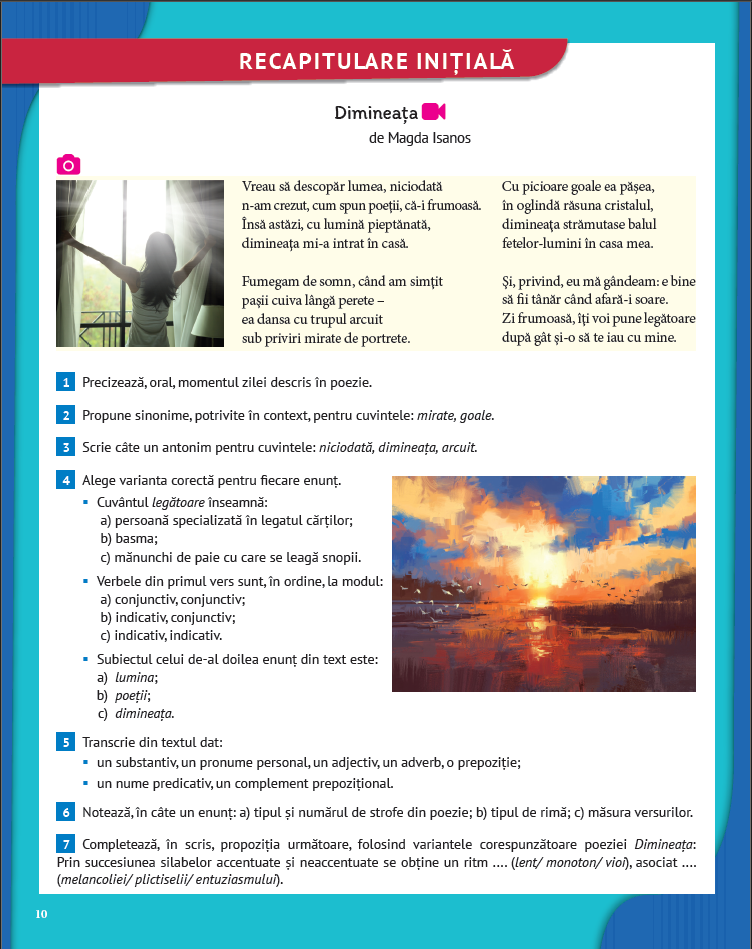
\includegraphics[width=.8\linewidth, height=.30\textheight]{Figura2_3a}
		\caption{pagină din manualul tipărit}
		\label{fig:Figura2_3a}
	\end{subfigure}%
	\begin{subfigure}{.5\textwidth}
		\centering
		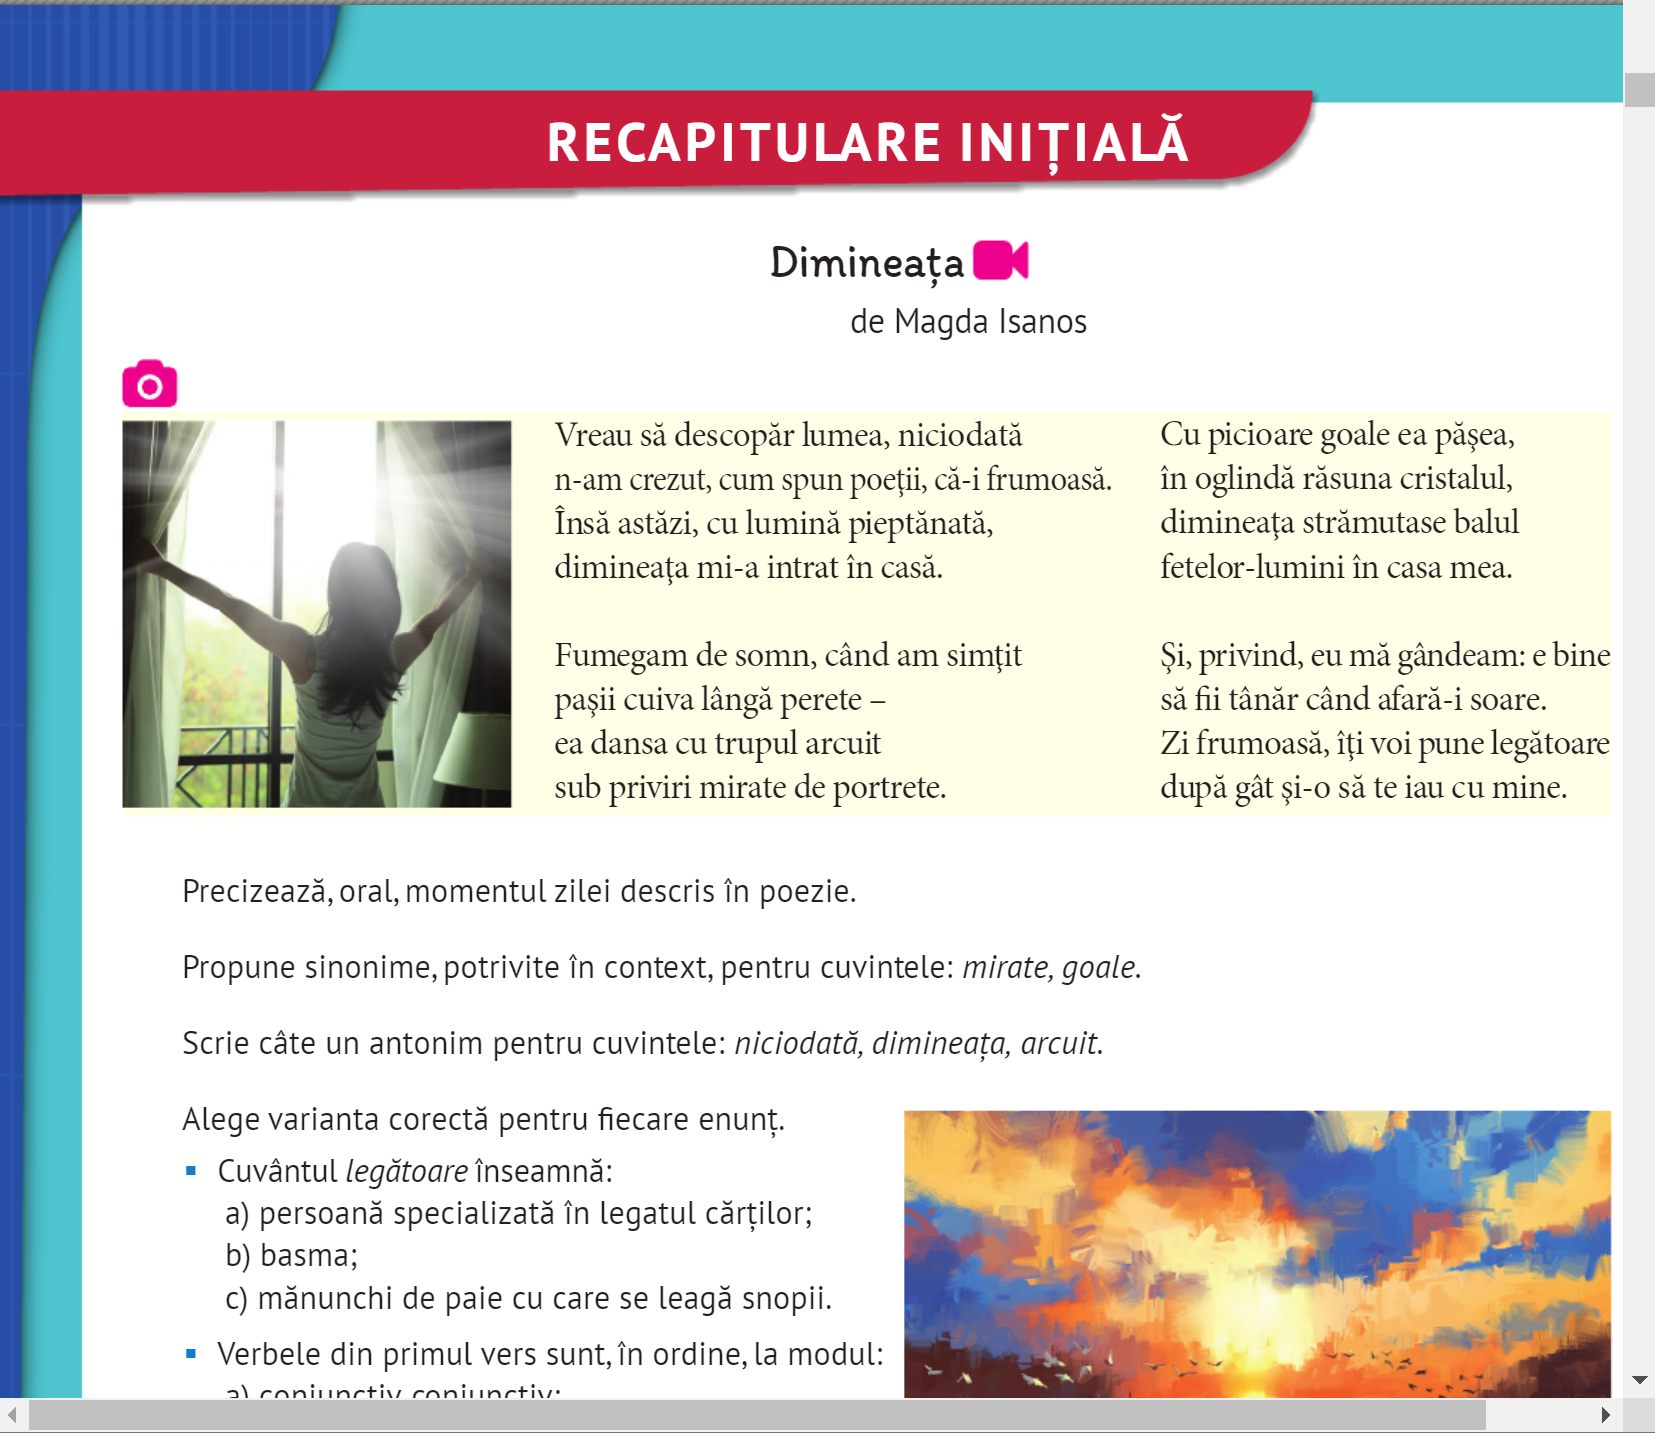
\includegraphics[width=.8\linewidth, height=.30\textheight]{Figura2_3b}
		\caption{pagină HTML generată de CloudConvert}
		\label{fig:Figura2_3b}
	\end{subfigure}
	\caption{Comparație de pagini dintre varianta tipărită și cea de la CloudConvert}
	\label{fig:Figura2_3}
\end{figure}

\noindent
Avantaje:
\begin{itemize}
	\item generează rapid pagini HTML;
	\item textul este selectabil;
	\item păstrează formatarea exact cum este în manualul tipărit;
	\item nu este limitat la un număr de utilizări.
\end{itemize}

\noindent
Dezavantaje:
\begin{itemize}
	\item paginile nu sunt responsive;
	\item codul HTML este greu de editat.
\end{itemize}

\section{HTML 4.01 Transitional}

O altă soluție găsită a fost extragerea textului din documentul PDF și plasarea acestuia într-un fișier de tip HTML 4.01 Transitional \cite{raggett1997html}. Deși acest format este mai simplu de utilizat și editat, el nu este la fel de modern ca HTML5.

Un exemplu de site care utilizează această metodă de conversie este PDF24 Tools. Avantajul principal este ușurința cu care se poate edita codul HTML. Totuși, site-ul nu păstrează formatul original al documentului PDF. Singurele atribute pe care le menține sunt stilurile de text bold și italic.
\begin{figure}[H]
	\centering
	\begin{subfigure}{.5\textwidth}
		\centering
		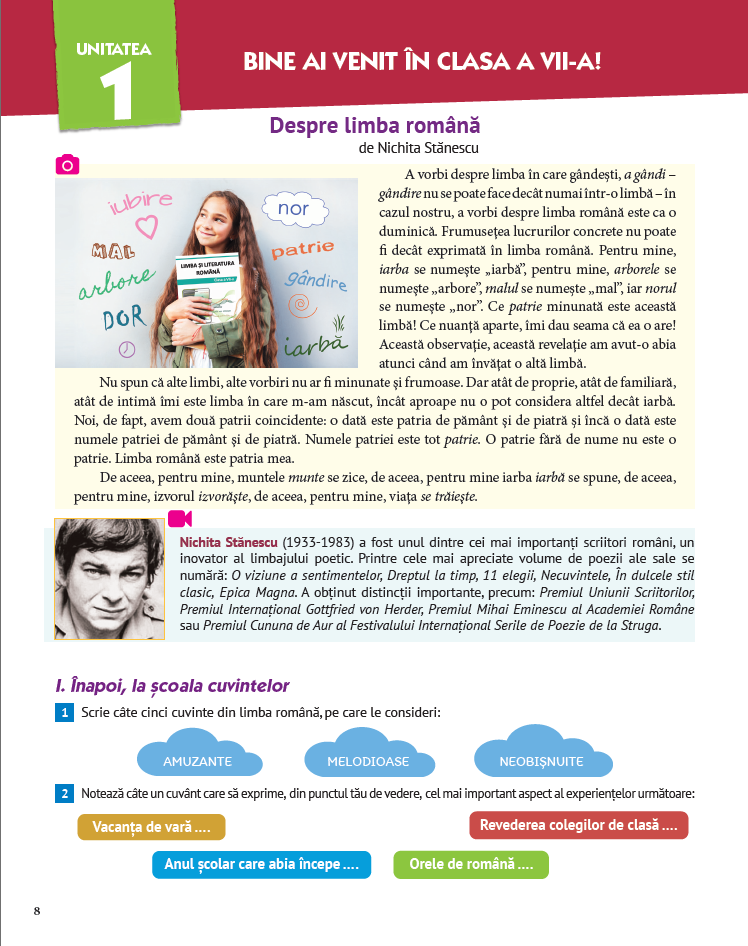
\includegraphics[width=.8\linewidth, height=.3\textheight]{Figura2_4a}
		\caption{pagină din manualul tipărit}
		\label{fig:Figura2_4a}
	\end{subfigure}%
	\begin{subfigure}{.5\textwidth}
		\centering
		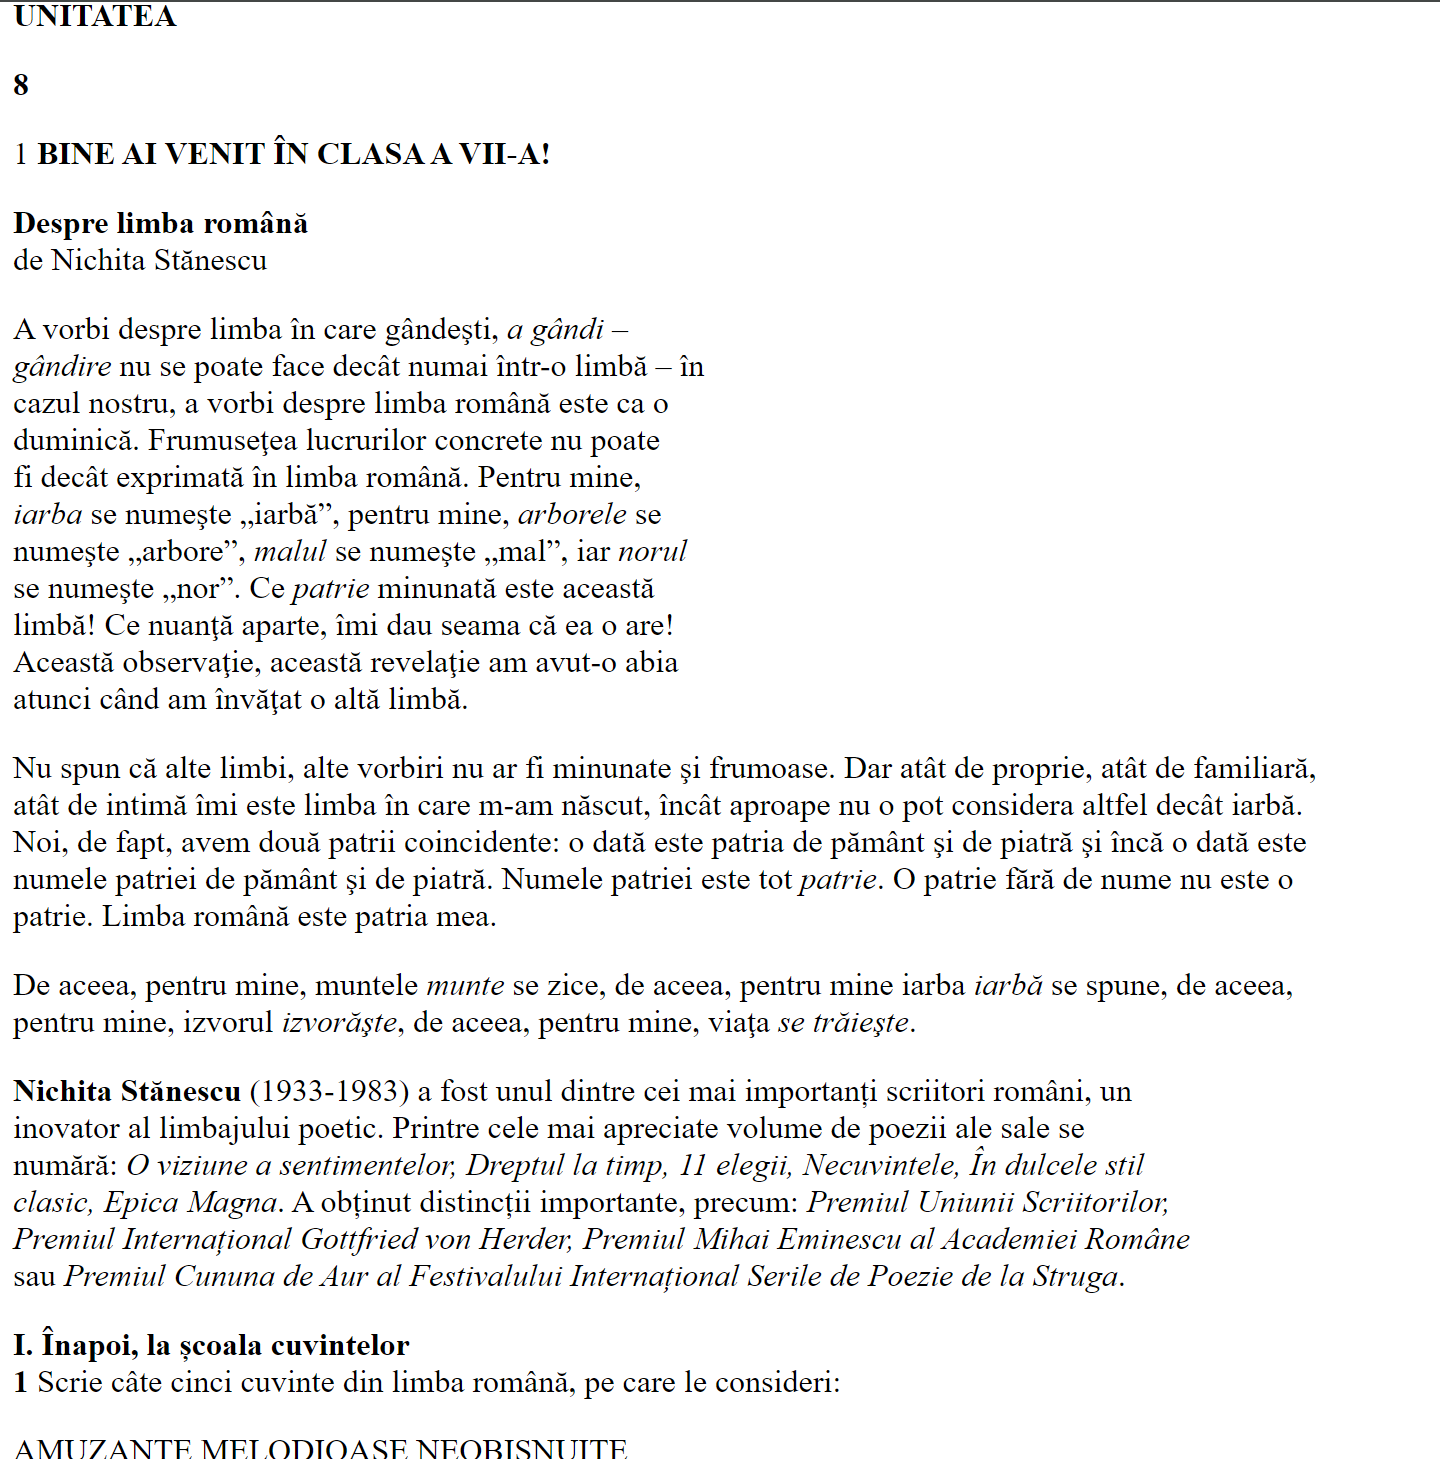
\includegraphics[width=.8\linewidth, height=.3\textheight]{Figura2_4b}
		\caption{pagină HTML generată de PDF24 Tools}
		\label{fig:Figura2_4b}
	\end{subfigure}
	\caption{Comparație de pagini dintre varianta tipărită și cea de la PDF24 Tools}
	\label{fig:Figura2_4}
\end{figure}

\noindent
Avantaje:
\begin{itemize}
	\item generează rapid pagini HTML;
	\item textul este selectabil;
	\item nu este limitat la un număr de utilizări;
	\item codul este ușor de editat.
\end{itemize}

\noindent
Dezavantaje:
\begin{itemize}
	\item păstrează doar o parte din formatarea originală (textul bold și italic).
\end{itemize}

\vspace{3em}
Necesitatea de a dezvolta încă un instrument de conversie a PDF-urilor în HTML provine din faptul că soluțiile actuale nu satisfac cerințele date de Minister. Niciuna dintre soluțiile analizate nu reprezintă un punct de plecare bun.

\begin{table}[H]
	\centering
	\begin{tabular}{| l | c | c | c | c |}
		\hline
		\textbf{Soluții/Criterii} & Selectabil & Responsive & Cod ușor de editat & Formatare corectă \\ \hline
		Conversia în imagini &  & $\times$ & $\times$ & $\times$ \\ \hline
		Xodo & $\times$ & $\times$ &  & \\ \hline
		pdf2htmlEX & $\times$ &  &  & $\times$ \\ \hline
		PDF24 Tools & $\times$ & $\times$ & $\times$ & \\ \hline
	\end{tabular}
	\caption{Comparație între instrumentele disponibile pe piață}
\end{table}